\documentclass{article}
\usepackage[landscape, margin=10mm, paper=a6paper, includehead, includefoot]{geometry}
\usepackage{lipsum}
\usepackage{graphicx}
\usepackage{multicol}
\usepackage{fancyhdr}
\usepackage{scrextend}
\usepackage{paralist}

\KOMAoptions{fontsize=8pt}
\setlength{\parindent}{0pt}
\raggedright

% Define fancy headers and footers
\pagestyle{fancy}
\fancyhf{}
\fancyhead[L]{\leftmark}
\fancyfoot[C]{\thepage}


%%%%%%%%%%%%% DOCUMENT START %%%%%%%%%%%%%
\begin{document}
\pagenumbering{gobble}

%%%%%%%%%%%%% FIRST PAGE %%%%%%%%%%%%%
\newpage
% HEADER:
\pagestyle{fancy}
\fancyhf{}                    %%%% REMOVING PRIOR HEAD AND FOOT
\fancyhead[L]{GMT}            %%%% HEAD LEFT SUBJECT
\fancyhead[C]{Werkstoffe}     %%%% HEAD MID TOPIC
\fancyhead[R]{Holz, Ökologie} %%%% HEAD RIGHT SUBTOPIC

% CONTENT START
\paragraph{Warum kann die Holzgewinnung ökologisch bedenklich sein?}
\begin{itemize}
\item Trotz der Tatsache, dass Holz ein nachwachsender Rohstoff ist, kann die
  Holzgewinnung problematisch sein. Beispiele hierfür sind übermäßige
  Abholzung, versäumte Wiederaufforstung, Plantagenwirtschaft in Monokulturen
  oder Bodenverdichtung. Insbesondere bei Tropenhölzern kann die Abholzung der
  Regenwälder oder die Holzgewinnung für die Papierindustrie durch Abholzen der
  großen kanadischen Urwälder ökologisch bedenklich sein.
\end{itemize}
% FOOTER:
\fancyfoot[L]{Daniel Renschler}
\fancyfoot[R]{J1-2}



% TEMPLATES:
%%%%%%%%%%%%% personal %%%%%%%%%%%%%
\newpage
% HEADER:
\pagestyle{fancy}
\fancyhf{}                    %%%% REMOVING PRIOR HEAD AND FOOT
\fancyhead[L]{subject}            %%%% HEAD LEFT SUBJECT
\fancyhead[C]{topic}     %%%% HEAD MID TOPIC
\fancyhead[R]{subtopic}         %%%% HEAD RIGHT SUBTOPIC

%TITLE:
\paragraph{title}
%CONTENT START
\begin{itemize}
\item content%CONTENT AS ITEM
\end{itemize}

% FOOTER:
\fancyfoot[L]{Daniel Renschler}
\fancyfoot[R]{J1-2}


%%%%%%%%%%%%%%%%%% VARIABLE CARD %%%%%%%%%%%%%%%%%%%%
\newpage
% HEADER:
\pagestyle{fancy}
\fancyhf{}                    %%%% REMOVING PRIOR HEAD AND FOOT
\fancyhead[L]{GMT}        %%%% HEAD LEFT SUBJECT
\fancyhead[C]{Werkstoffe}          %%%% HEAD MID TOPIC
\fancyhead[R]{Holz, Spahnholz}       %%%% HEAD RIGHT SUBTOPIC


% TESTING MULTICOL
\begin{multicols}{3}
  \paragraph{Sperrholz:}
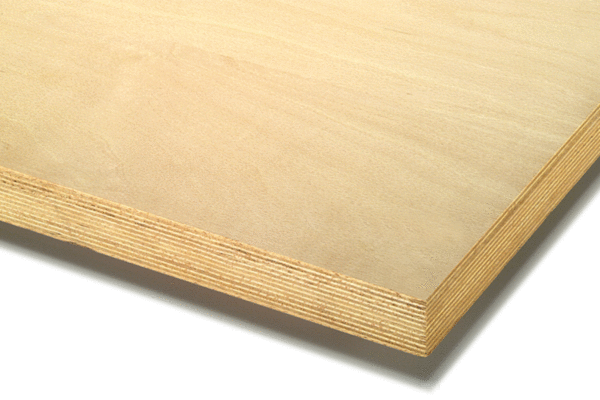
\includegraphics[width=\linewidth]{sperrh.png}
Dichte: 0,5-0,9$\frac{g}{cm^3}$
Zugfestigkeit: 6-10 $\frac{N}{mm^2}$, flach.

Werden durch verkleben von Furnieren, Spähnen, und Holzfasern Hergestellt.\\
Gewinnung sehr einfach im Vergleich zu Vollholz, da alles vom Baum verwendet werden kann.

Hergestellt aus unterschiedlich großen Spähnen, meist 3-5 Schichten verleimt und verpresst.\\
-Wesentlich geringere Stärke als Festholz.

Verwendung:
\begin{compactitem}
  \item Möbel-
  \item Fahrzeugs-
  \item Bootsbau-
  \item Verpackungsmaterial
\end{compactitem}

Verwertung:
\begin{compactitem}
  \item schwer recyclebar durch Kunstoffharzanteile (Filteranlagen notwendig)
  \item geschlossener $CO_2$ Kreislauf (gebundenes $CO_2$ wird wieder frei.)
\end{compactitem}

Entsorgung:
\begin{compactitem}
  \item Holzanteil kann mit der Zeit verotten
  \item Wird verbrannt, zerkleinert, oder zu Spähnen verarbeitet.
\end{compactitem}

\end{multicols}

\fancyfoot[L]{Daniel Renschler}
\fancyfoot[R]{J1-2}

\end{document}
